\documentclass{article}

\usepackage[T1]{fontenc}
\usepackage[utf8]{inputenc}
\usepackage{graphicx}
\usepackage{polski}
\usepackage{listings}
\usepackage{xcolor}

\colorlet{punct}{red!60!black}
\definecolor{background}{HTML}{EEEEEE}
\definecolor{delim}{RGB}{20,105,176}
\colorlet{numb}{magenta!60!black}

\newcommand{\mparagraph}[1]{\paragraph{#1}\mbox{}\vspace{2mm}\\}

\lstdefinelanguage{json}{
    basicstyle=\normalfont\ttfamily,
    numbers=left,
    numberstyle=\scriptsize,
    stepnumber=1,
    numbersep=8pt,
    showstringspaces=false,
    breaklines=true,
    frame=lines,
    literate=
     *{0}{{{\color{numb}0}}}{1}
      {1}{{{\color{numb}1}}}{1}
      {2}{{{\color{numb}2}}}{1}
      {3}{{{\color{numb}3}}}{1}
      {4}{{{\color{numb}4}}}{1}
      {5}{{{\color{numb}5}}}{1}
      {6}{{{\color{numb}6}}}{1}
      {7}{{{\color{numb}7}}}{1}
      {8}{{{\color{numb}8}}}{1}
      {9}{{{\color{numb}9}}}{1}
      {:}{{{\color{punct}{:}}}}{1}
      {,}{{{\color{punct}{,}}}}{1}
      {int}{{{\color{magenta}{int}}}}{3}
      {string}{{{\color{magenta}{string}}}}{6}
      {boolean}{{{\color{magenta}{boolean}}}}{7}
      {"}{{{\color{numb}{"}}}}{1}
      {\{}{{{\color{delim}{\{}}}}{1}
      {\}}{{{\color{delim}{\}}}}}{1}
      {[}{{{\color{delim}{[}}}}{1}
      {]}{{{\color{delim}{]}}}}{1},
}

\title{Sprawozdanie z projektu - Poker Royal Flush}
\author{Artur Prasuła}

\begin{document}
\maketitle
\tableofcontents
\newpage


\section{Opis tematyki projektu}
    Moim zadaniem było stworzenie systemu do gry w pokera.
    System ten najpierw został przeze mnie zaprojektowany, a następnie zaimplementowany w języku Java.
    W skład tego systemu wchodziła aplikacja kliencka oraz aplikacja serwerowa.
    
    \subsection{Klient}
        Klient działa jako aplikacja desktopowa na komputery PC.
        Został on wykonany przy użyciu technologii \textbf{JavaFX}.
        Zastosowany został tzw. lekki klient, czyli klient z jak najmniejszą liczbą zadań.
        Aplikacja ta służy jako interfejs komunikacji pomiędzy graczem, a serwerem.
    
    \subsection{Serwer}
        Serwer został zaimplementowany w języku \textbf{Java}.
        Aplikacja serwerowa pozwala na połączenie z bazą danych, dzięki czemu stan graczy jest zapisany w pamięci pomimo, że gracze nie są dostępni na serwerze.
        Jest to funkcja dodatkowa i serwer działa poprawnie nawet jeśli nie udało się połączyć z bazą danych.

\section{Sposób użycia}

    \subsection{Klient}
        Klient jest aplikacją wyposażoną w graficzny interfejs użytkownika.
        Uruchamiamy go jak każdy inny taki program - na przykład klikając podwójnie w ikonę aplikacji.
        
        \begin{center}
            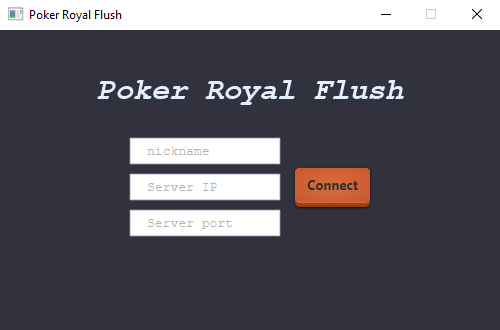
\includegraphics[width=75mm]{ekran_start.png}
            \\
            Ekran startowy aplikacji klienckiej
        \end{center}
        
        W tym miejscu podajemy dane potrzebne do połączenia się z serwerem.
        Po naciśnięciu przycisku ,,Connect'' aplikacja wykona próbę połączenia się.
        Jeśli ta próba zakończy się niepowodzeniem zostanie wyświetlony odpowiedni komunikat.
        W przeciwnym wypadku, aplikacja zmieni scenę na scenę główną - tą z widokiem stołu.
        
        \vspace{4mm}
        
        \begin{center}
            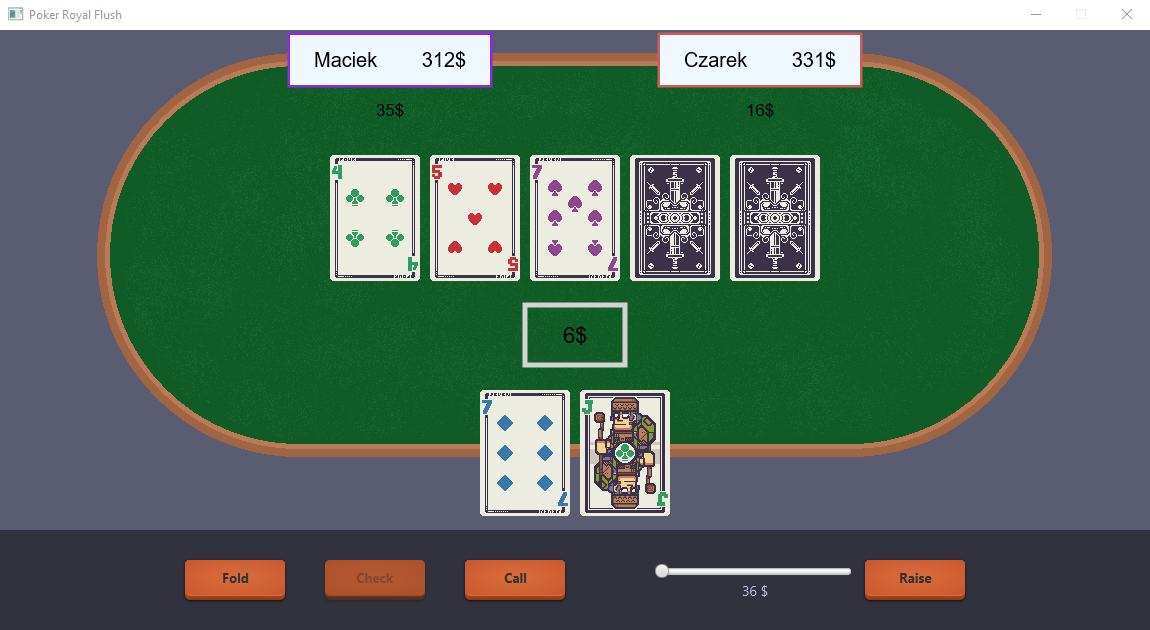
\includegraphics[width=\textwidth]{ekran_glowny.png}
            \\
            Ekran główny aplikacji klienckiej
        \end{center}
    
        Ekran główny służy do brania udziału w rozgrywce.
        To na tym ekranie będziemy widzieć jej stan.
        Ta scena również służy graczowi do wykonywania ruchów.
        Odpowiednie przyciski odblokowują się w sytuacji gdy gracz może wykonać dany ruch.
       
    
    \subsection{Serwer}
        Serwer nie jest wyposażony w graficzny interfejs użytkownika gdyż taki nie jest potrzebny.
        Aplikacja po uruchomieniu nie wymaga żadnej ingerencji.
        Bardzo ważna jest natomiast konfiguracja startowa aplikacji.
        W skład tej konfiguracji wchodzi: parametry uruchomienne serwera, konfiguracja połączenia z bazą danych.\\
        \\
        \textbf{Parametry uruchomienne}
            \begin{center}
                java -jar PokerRoyalFlushServer.jar [port] [start money] [blind]
            \end{center}
            gdzie,\\
            \textbf{port} - port serwera (domyślnie - 5000)\\
            \textbf{start money} - wartość początkowej ilości pieniędzy jaką dostaje każdy z gracz po dołączeniu do stołu (domyślnie - 200)\\
            \textbf{blind} - wartość ciemnej (domyślnie - 1)\\
        \\
        \textbf{Konfiguracja połączenia z bazą danych}\\
            Do skonfigurowania połączenia serwera mojej aplikacji z serwerem bazy danych wykorzystywany jest plik konfiguracyjny \textbf{database.config} w którym definiujemy wszystkie potrzebne do połączenia dane.\\
            Plik \textbf{database.config}:
            
            \begin{lstlisting}[language=json, firstnumber=1]
database.url=url
database.username=login
database.password=haslo
            \end{lstlisting}
            \vspace{2mm}
            
            Jeżeli plik konfiguracyjny będzie zawierać jakieś błędy lub taki plik nie będzie istnieć aplikacja poinformuje użytkownika o błędzie.
            Implementacja serwera przewiduje w takiej sytuacji dalsze działanie serwera z nieaktywną funkcjonalnością bazy danych.
        

\section{Opis struktury projektu}


\section{Testowanie programu i wyniki}


\section{Zmiany względem specyfikacji}


\section{Wnioski i spostrzeżenia}


\end{document}